\documentclass[a4paper,10pt]{article}

% engine-related
\usepackage{etoolbox}
\usepackage{ifxetex}
\usepackage{ifluatex}

\ifboolexpr { bool {luatex} or bool {xetex} } 
{
    % modern packages, highly recommended
    \usepackage{fontspec}
    \defaultfontfeatures{Mapping=tex-text,Ligatures=TeX}
    \usepackage[backend=biber,style=numeric]{biblatex}
} 
{
    % legacy packages
    \usepackage[T1]{fontenc}
    \usepackage[utf8]{inputenc}
    \usepackage{graphicx}
    \usepackage{epstopdf}
    \usepackage[backend=bibtex, style=numeric]{biblatex}
}


\addbibresource{references/bibliography.bib}

\usepackage[inner=3cm,top=3cm,outer=3cm,bottom=3cm]{geometry}
\usepackage[parfill]{parskip}

\usepackage[toc,page]{appendix}
\usepackage{csquotes}
\usepackage{amsmath}
\usepackage{amssymb}
\usepackage{amsthm}
\usepackage{mathtools}
\usepackage{verbatim}
\usepackage{algpseudocode}
\usepackage{float}
\usepackage{tikz}
\usetikzlibrary{decorations.pathreplacing}
\usepackage{mathtools}
\usepackage{enumitem}
\usepackage{calc}
\usepackage{multido}

\usepackage{caption}
\usepackage{subcaption}
\usepackage{hyperref}

\usepackage[ireport, eng]{pkg/KTHEEtitlepage}
\DeclarePairedDelimiter\ceil{\lceil}{\rceil}
\DeclarePairedDelimiter\floor{\lfloor}{\rfloor}

\newcommand{\cauthor}{André Nyström \& Axel Riese}
\newcommand{\ctitle}{Algorithms and Complexity for Video and Computer Games}
\newcommand{\csubtitle}{A Lumines survey}
\newcommand{\cdate}{\today}
\newcommand{\caddress}
{
    Degree Project in Computer Science, DD143X \\
    Examinator: Örjan Ekeberg
}

\newcommand{\lummonowhite}[2]
{
    \filldraw[fill=white, draw=black] (#1,#2) rectangle (#1+1,#2+1);
    \filldraw[fill=white, draw=black] (#1+1,#2) rectangle (#1+2,#2+1);
    \filldraw[fill=white, draw=black] (#1,#2+1) rectangle (#1+1,#2+2);
    \filldraw[fill=white, draw=black] (#1+1,#2+1) rectangle (#1+2,#2+2);
}

\newcommand{\lummonoblack}[2]
{
    \filldraw[fill=gray, draw=black] (#1,#2) rectangle (#1+1,#2+1);
    \filldraw[fill=gray, draw=black] (#1+1,#2) rectangle (#1+2,#2+1);
    \filldraw[fill=gray, draw=black] (#1,#2+1) rectangle (#1+1,#2+2);
    \filldraw[fill=gray, draw=black] (#1+1,#2+1) rectangle (#1+2,#2+2);
}

\newcommand{\lumlwhite}[2]
{
    \filldraw[fill=white, draw=black] (#1,#2) rectangle (#1+1,#2+1);
    \filldraw[fill=white, draw=black] (#1+1,#2) rectangle (#1+2,#2+1);
    \filldraw[fill=gray, draw=black] (#1,#2+1) rectangle (#1+1,#2+2);
    \filldraw[fill=white, draw=black] (#1+1,#2+1) rectangle (#1+2,#2+2);
}

\newcommand{\lumh}[2]
{
    \filldraw[fill=white, draw=black] (#1,#2) rectangle (#1+1,#2+1);
    \filldraw[fill=gray, draw=black] (#1+1,#2) rectangle (#1+2,#2+1);
    \filldraw[fill=white, draw=black] (#1,#2+1) rectangle (#1+1,#2+2);
    \filldraw[fill=gray, draw=black] (#1+1,#2+1) rectangle (#1+2,#2+2);
}

\newcommand{\lumlblack}[2]
{
    \filldraw[fill=gray, draw=black] (#1,#2) rectangle (#1+1,#2+1);
    \filldraw[fill=gray, draw=black] (#1+1,#2) rectangle (#1+2,#2+1);
    \filldraw[fill=white, draw=black] (#1,#2+1) rectangle (#1+1,#2+2);
    \filldraw[fill=gray, draw=black] (#1+1,#2+1) rectangle (#1+2,#2+2);
}

\newcommand{\lumx}[2]
{
    \filldraw[fill=gray, draw=black] (#1,#2) rectangle (#1+1,#2+1);
    \filldraw[fill=white, draw=black] (#1+1,#2) rectangle (#1+2,#2+1);
    \filldraw[fill=white, draw=black] (#1,#2+1) rectangle (#1+1,#2+2);
    \filldraw[fill=gray, draw=black] (#1+1,#2+1) rectangle (#1+2,#2+2);
}


\newcommand{\stripew}[2]
{
    \cellw{#1}{#2}
    \cellb{#1+1}{#2}
    \cellw{#1+2}{#2}
    \cellb{#1+3}{#2}
}

\newcommand{\stripeb}[2]
{
    \cellb{#1}{#2}
    \cellw{#1+1}{#2}
    \cellb{#1+2}{#2}
    \cellw{#1+3}{#2}
}

\newcommand{\wellbot}[2]
{
    \stripew{#1}{#2}
    \cellb{#1}{#2+1}
    \cellw{#1+1}{#2+1}
    \cellw{#1+2}{#2+1}
    \cellb{#1+3}{#2+1}
}

\newcommand{\toprow}[2]
{
    \cellb{#1}{#2}
    \cellw{#1+1}{#2}
    \cellb{#1+2}{#2}
    \cellb{#1+3}{#2}
}

\newcommand{\topblock}[2]
{
    \stripew{#1}{#2}
    \toprow{#1}{#2+1}
}

\newcommand{\welltop}[2]
{
    \topblock{#1}{#2}
    \topblock{#1}{#2+2}
}

\newcommand{\wellclosed}[2]
{
    \cellw{#1}{#2}
    \cellb{#1}{#2+1}
    \cellw{#1+3}{#2}
    \cellw{#1+3}{#2+1}
}

\newcommand{\wellopen}[2]
{
    \cellw{#1}{#2}
    \cellb{#1+1}{#2}
    \cellb{#1}{#2+1}
    \cellb{#1+1}{#2+1}
}

\newcommand{\welldefault}[2]
{
    \wellbot{#1}{#2}
    \draw[dotted] (#1+2, #2+2) -- (#1+2, #2+4);
    \welltop{#1}{#2+4}
    \wellclosed{#1}{#2+8}
}

\newcommand{\wellopenwhole}[2]
{
    \wellbot{#1}{#2}
    \draw[dotted] (#1+2, #2+2) -- (#1+2, #2+4);
    \welltop{#1}{#2+4}
    \wellopen{#1}{#2+8}
}

\newcommand{\welldetailed}[2]
{
    \wellbot{#1}{#2}
    \draw[dotted] (#1+2, #2+2) -- (#1+2, #2+4);
    \wellbot{#1}{#2+4}
    \topblock{#1}{#2+6}
    \draw[dotted] (#1+2, #2+8) -- (#1+2, #2+10);
    \welltop{#1}{#2+10}
    \wellclosed{#1}{#2+14}
}

\newcommand{\topclosed}[2]
{
    \draw[dotted] (#1+2, #2) -- (#1+2, #2+2);
    \welltop{#1}{#2+2}
    \wellclosed{#1}{#2+6}
}

\newcommand{\topopen}[2]
{
    \draw[dotted] (#1+2, #2) -- (#1+2, #2+2);
    \welltop{#1}{#2+2}
    \wellopen{#1}{#2+6}
}

\newcommand{\startb}[2]
{
    \cellb{#1}{#2}
    \cellw{#1+1}{#2}
    \cellb{#1}{#2+1}
    \cellw{#1+1}{#2+1}
}

\newcommand{\middleb}[2]
{
    \cellw{#1}{#2}
    \cellb{#1+1}{#2}
    \cellw{#1}{#2+1}
    \cellb{#1+1}{#2+1}
}

\newcommand{\ponemid}[2]
{
    \cellw{#1}{#2}
    \cellb{#1+1}{#2}
    \cellw{#1+2}{#2}
    \cellw{#1+3}{#2}
    \stripeb{#1}{#2+1}
}

\newcommand{\invariantchart}[2]
{
    \wellbot{#1}{#2}
    \draw[dotted] (#1+2, #2+2) -- (#1+2, #2+4);
    \wellbot{#1}{#2+4}
    \topblock{#1}{#2+6}
    \draw[dotted] (#1+2, #2+8) -- (#1+2, #2+10);
    \topblock{#1}{#2+10}
    \ponemid{#1}{#2+12}
    \draw[dotted] (#1+2, #2+14) -- (#1+2, #2+16);
    \ponemid{#1}{#2+16}
    \ponemid{#1}{#2+18}
    \wellclosed{#1}{#2+20}
}

\newcommand{\stopb}[2]
{
    \cellw{#1}{#2}
    \cellb{#1+1}{#2}
    \cellb{#1}{#2+1}
    \cellw{#1+1}{#2+1}
}

\newcommand{\ptwoopen}[2]
{
    \draw[dotted] (#1+2, #2) -- (#1+2, #2+2);
    \ponemid{#1}{#2+2}
    \ponemid{#1}{#2+4}
    \wellopen{#1}{#2+6}
}

\newcommand{\ptwoclosed}[2]
{
    \draw[dotted] (#1+2, #2) -- (#1+2, #2+2);
    \ponemid{#1}{#2+2}
    \ponemid{#1}{#2+4}
    \wellclosed{#1}{#2+6}
}

\newcommand{\pthreeone}[2]
{
    \draw[dotted] (#1+2, #2) -- (#1+2, #2+2);
    \ponemid{#1}{#2+2}
    \ponemid{#1}{#2+4}
    \cellw{#1}{#2+6}
    \cellb{#1}{#2+7}
}

\newcommand{\checkbox}[2]
{
    \stripew{#1}{#2}
    \stripeb{#1}{#2+1}
}

\newcommand{\wellblocked}[2]
{
    \cellw{#1}{#2}
    \cellb{#1+1}{#2}
    \cellw{#1+2}{#2}
    \cellb{#1}{#2+1}
    \cellw{#1+1}{#2+1}
    \cellb{#1+2}{#2+1}
}

\newcommand{\beforecollapse}[2]
{
    \wellbot{#1}{#2}
    \draw[dotted] (#1+2, #2+2) -- (#1+2, #2+4);
    \wellbot{#1}{#2+4}
    \ponemid{#1}{#2+6}
    \draw[dotted] (#1+2, #2+8) -- (#1+2, #2+10);
    \ponemid{#1}{#2+10}
    \checkbox{#1}{#2+12}
    \draw[dotted] (#1+2, #2+14) -- (#1+2, #2+16);
    \checkbox{#1}{#2+16}
    \checkbox{#1}{#2+18}
    \wellblocked{#1}{#2+20}
}

\newcommand{\collapsepre}[2]
{
    \wellbot{#1}{#2}
    \draw[dotted] (#1+2, #2+2) -- (#1+2, #2+4);
    \checkbox{#1}{#2+4}
    \checkbox{#1}{#2+6}
    \cellr{#1+2}{#2+4}
    \cellr{#1+3}{#2+4}
    \cellr{#1+2}{#2+5}
    \cellr{#1+3}{#2+5}
    \cellr{#1+2}{#2+6}
    \cellr{#1+3}{#2+6}
    \draw[dotted] (#1+2, #2+8) -- (#1+2, #2+10);
    \checkbox{#1}{#2+10}
    \checkbox{#1}{#2+12}
    \draw[dotted] (#1+2, #2+14) -- (#1+2, #2+16);
    \checkbox{#1}{#2+16}
    \checkbox{#1}{#2+18}
    \wellblocked{#1}{#2+20}
}

\newcommand{\collapsemid}[2]
{
    \cellw{#1}{#2}
    \cellb{#1+1}{#2}
    \cellb{#1+2}{#2}
    \cellw{#1+3}{#2}

    \cellb{#1}{#2+1}
    \cellw{#1+1}{#2+1}
    \cellw{#1+2}{#2+1}
    \cellw{#1+3}{#2+1}
}

\newcommand{\collapsetop}[2]
{
    \cellw{#1}{#2}
    \cellb{#1+1}{#2}
    \cellb{#1+2}{#2}
    \cellw{#1+3}{#2}

    \cellb{#1}{#2+1}
    \cellw{#1+1}{#2+1}
    \cellw{#1+2}{#2+1}
    \cellb{#1+3}{#2+1}
}

\newcommand{\collapsehat}[2]
{
    \cellw{#1}{#2}
    \cellb{#1+1}{#2}
    \cellb{#1+2}{#2}
    \cellw{#1+3}{#2}

    \cellb{#1}{#2+1}
    \cellw{#1+1}{#2+1}
    \cellw{#1+2}{#2+1}

    \cellw{#1}{#2+2}
    \cellb{#1+1}{#2+2}
    \cellb{#1+2}{#2+2}

    \cellb{#1}{#2+3}
    \cellw{#1+1}{#2+3}

    \cellw{#1}{#2+4}
    \cellb{#1+1}{#2+4}

    \cellb{#1}{#2+5}
    \cellw{#1+1}{#2+5}
}

\newcommand{\collapsepost}[2]
{
    \wellbot{#1}{#2}
    \draw[dotted] (#1+2, #2+2) -- (#1+2, #2+4);
    \collapsemid{#1}{#2+4}
    \collapsemid{#1}{#2+6}
    \draw[dotted] (#1+2, #2+8) -- (#1+2, #2+10);
    \collapsetop{#1}{#2+10}
    \collapsetop{#1}{#2+12}
    \draw[dotted] (#1+2, #2+14) -- (#1+2, #2+16);
    \collapsehat{#1}{#2+16}
}

\theoremstyle{plain}
\newtheorem{thm}{Theorem}[section] % reset theorem numbering for each chapter

\theoremstyle{plain}
\newtheorem{lem}[thm]{Lemma} % same for example numbers
\newtheorem{cor}[thm]{Corollary} % same for example numbers

\theoremstyle{definition}
\newtheorem{defn}[thm]{Definition} % definition numbers are dependent on theorem numbers
\newtheorem{exmp}[thm]{Example} % same for example numbers

\begin{document}
\ititle{\ctitle}
\isubtitle{\csubtitle}
\iauthor{\cauthor}
\idate{\today}
%\irefnr{IR-EE-Dummy 2000:099}

\iaddress{\caddress}
\makeititle

\tableofcontents
\newpage

\section{Introduction}

In this report a simplified version of the game Lumines is shown to be NP-complete. First the rules of the game are formally defined. Using these definitions the NP-complete subset sum problem is reduced to a Lumines gameboard with a defined sequence of blocks. A proof is presented showing that the only way to clear a specific number of blocks in the given Lumines gameboard is if the subset sum instance is a ``yes''-instance.

\subsection{The game}
The video game Lumines was released in December 2004 in Japan for the PSP platform. The game was a major success for the developer Q Entertainment, and has since its original release been followed with a couple of sequels \cite{wiki:lumines}.
\begin{figure}[H]
    \centering
    \resizebox{0.7\textwidth}{!}{
    
\begin{tikzpicture}
        \lummonowhite{0}{0}
        \lummonoblack{3}{0}
        \lumlwhite{6}{0}
        \lumlblack{9}{0}
        \lumh{12}{0}
        \lumx{15}{0}
    \end{tikzpicture}
    }
    \caption{The six pieces of lumines: M\{W,B\}, L\{W,B\}, H and X}
    \label{fig:pieces}
\end{figure}

Lumines is a two-dimensional grid game, in which a sequence of $2 \times 2$ dichromatic \textit{blocks} falls, and the user rotates and shifts the block before its bottom \text{cells} reaches other cells, \textit{terrain}, in the gameboard. When the block reach existing terrain, it is no longer possible to shift or rotate the block. If both bottom cells of the block is supported by existing terrain, the block stays put on that terrain. Otherwise, the half of the block that is not supported by terrain will fall down until it is. The player is then presented with the next block.

\begin{figure}[H]
    \centering
    \resizebox{0.7\textwidth}{!}{
    \begin{subfigure}[b]{0.45\linewidth}
        \resizebox{\linewidth}{!}{
        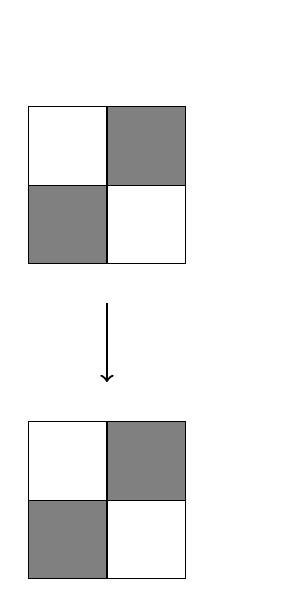
\begin{tikzpicture}
            \lumx{0}{4}
            \draw[thick, ->] (1,3.5) -- (1, 2.5);
            \lumx{0}{0}
            \draw [draw=none] rectangle (3, 7);
        \end{tikzpicture}
        \hspace{0.25cm}
        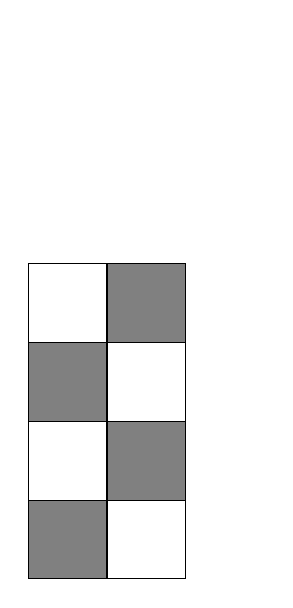
\begin{tikzpicture}
            \lumx{0}{2}
            \lumx{0}{0}
            \draw [draw=none] rectangle (3, 7);
        \end{tikzpicture}
        }
        \caption{}
    \end{subfigure}
    \hspace{0.05\linewidth}
    \begin{subfigure}[b]{0.45\linewidth}
        \resizebox{\linewidth}{!}{
        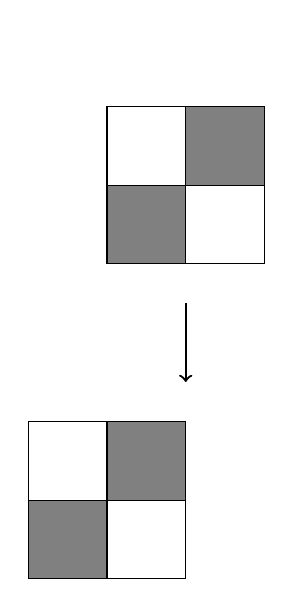
\begin{tikzpicture}
            \lumx{1}{4}
            \draw[thick, ->] (2,3.5) -- (2, 2.5);
            \lumx{0}{0}
            \draw [draw=none] rectangle (3, 7);
        \end{tikzpicture}
        \hspace{0.25cm}
        
\begin{tikzpicture}
            \lumx{0}{0}
            \cellb{1}{2}
            \cellw{1}{3}
            \cellw{2}{0}
            \cellb{2}{1}
            \draw [draw=none] rectangle (3, 7);
        \end{tikzpicture}
        }
        \caption{}
    \end{subfigure}
    }
    \caption{Block behavior with and without supporting terrain}
\end{figure}

If at any point the player forms a monochromatic $2 \times 2$ square, all cells belonging to that square is \textit{marked}. Note that these squares may overlap, for example all cells within a monochromatic $2 \times 3$ rectangle is marked, since it consists of overlapping $2 \times 2$ monochromatic squares. At a regular pace a vertical \textit{sweep-line} scans the gameboard and removes all marked cells.

\begin{figure}[H]
    \centering
    \resizebox{0.7\textwidth}{!}{
        \begin{subfigure}[b]{.3\linewidth}
        \fbox{
        \begin{tikzpicture}
            \cellw{0}{0}
            \cellw{1}{0}
            \cellb{2}{0}
            \cellw{0}{1}
            \cellw{2}{1}
            \cellw{2}{2}
            \cellb{0}{5}
            \cellw{1}{5}
            \cellb{0}{6}
            \cellw{1}{6}
            \draw [draw=none] (0,0) rectangle (3, 8);
        \end{tikzpicture}
        }
        \end{subfigure}
        \begin{subfigure}[b]{.3\linewidth}
        \fbox{
        \begin{tikzpicture}
            \cellw{0}{0}
            \cellw{1}{0}
            \cellb{2}{0}
            \cellw{0}{1}
            \cellw{2}{1}
            \cellw{2}{2}
            \cellb{0}{2}
            \cellw{1}{1}
            \cellb{0}{3}
            \cellw{1}{2}
            \draw [draw=none] (0,0) rectangle (3, 8);
        \end{tikzpicture}
        }
        \end{subfigure}
        \begin{subfigure}[b]{.3\linewidth}
        \fbox{
        
\begin{tikzpicture}
            \cellb{0}{2}
            \cellb{0}{3}
            \cellb{2}{0}
            \draw (0,0) [very thick, draw=black, fill=red] rectangle (2,2);
            \draw (1,1) [very thick, draw=black, fill=red] rectangle (3,3);
            \draw (1,1) [very thick, draw=black, fill=red] rectangle (2,2);
            \draw [draw=none] (0,0) rectangle (3, 8);
        \end{tikzpicture}
        }
        \end{subfigure}
    }
    \caption{Marking of $2 \times 2$ monochromatic squares (from \cite{lumines})}
\end{figure}

The version of Lumines found in the actual video games is played on a $10 \times 16$-gameboard. The goal of the standard game mode in Lumines is to survive, to keep placing blocks inside the gameboard, for as long as possible and clear as much terrain as possible in the process. The blocks given to the player is generated randomly, and 3-block lookahead is provided. The game starts on partially filled gameboard, which varies in size depending on the difficulty level \cite{lumines}.

\subsection{Problem statement}
This report considers the generalized version of the game, which is played on an $n \times m$-gameboard. The authors seek to formalize and  simplify Lumines, and explore this new system's computational complexity characteristics. Certain goals of the game are considered by translating them into decision problems in this system.

While the sweep-line is a core characteristic of Lumines, this report considers all marked terrain as instantly cleared. Furthermore the whole sequence of blocks is considered to be known beforehand. This will be referred to as the \textit{offline} version of the game, in contrast to the \textit{online} version, where the blocks are generated probabilistically as in the actual video game. These are the two main simplifications, although a more thorough discussion is provided in \nameref{method}. The impact of these simplifications on the validity of the results is considered in \nameref{discussion}.

The main Lumines goals this paper examines are:
\begin{itemize}
        \item Is (standard mode) Lumines NP-complete?
        \item Are all game modes of Lumines equally hard?
\end{itemize}

\subsection{Motivation}

Lumines is a game of interest because to the authors' knowledge it's not well researched from the perspective of computational complexity. Several similar games has been more thoroughly researched in recent years and comparing Lumines to these findings might yield interesting results. New findings on the computational complexity of Lumines may aid in the development of video game artificial intelligence. Our understanding of computational complexity in generic 2-dimensional grid games may also benefit from this research. Combining results from this report with results from previous similar research might make it possible to find a correlation between certain game characteristics and classes of computational complexity.

\section{Background}
\label{sec:background}

\subsection{Reduction}
A reduction is an algorithm used to solve one problem with another. A reduction of a decision problem is valid if each yes-instance gives a yes-instance and each no instance gives a no instance. If the reduction is to be made in polynomial time the problem that is solved must not be harder than the problem we reduce to.\cite{reduction}

\subsection{NP and PSPACE}
NP is the complexity class of all decision problems where a yes-instance can be verified in polynomial time. If it is possible to reduce all problems in NP to a certain problem, that problem is said to be NP-hard. A problem is referred to as a NP-complete problem if it is shown that it is both in NP and NP-hard. From this follows that if it is possible to reduce a NP-complete problem to some problem in NP using polynomial time, that problem is NP-complete as well.

PSPACE is the complexity class of all decision problems that can be solved by a Turing machine in a polynomial amount of memory space. Similar to NP-complete, a problem is PSPACE-complete if it is in PSPACE and all other problems in PSPACE can be reduced to the problem.

\subsection{The Subset Sum problem}

The \textit{Subset Sum} Problem is defined as follows \cite[p.~491]{algorithm}:

\begin{quote}
Given natural numbers $w_1, \ldots, w_n$, and a target number $W$, is there a subset of $\{w_1, \ldots, w_n \}$ that adds up precisely to $W$?
\end{quote}

The Subset Sum Problem plays a crucial role in this report; it is the chosen tproblem to reduce to the Lumines problem. It is known to be NP-complete \cite[p.~492]{algorithm}. In fact it is a special case of the Knapsack Problem \cite[p.~491]{algorithm}, one of Karp's 21 NP-complete problems he discusses in his 1972 paper \cite{karp}.

\subsection{Previous studies}
\subsubsection{Classical Nintendo Games}

In the paper on Classical Nintendo Games the computational complexity of games in the popular Nintendo series Legend of Zelda, Mario, Metroid, Donkey Kong and Pokémon are proven to be either NP- or PSPACE-hard \cite{classic}. The paper states that it is easy to understand that most games are members of PSPACE because their behaviour is a deterministic function of the player's controller input. The paper focus on the reachability problem in the aforementioned games, that is if it is possible to get from point A to point B on a generalized gameboard. Using the NP-complete problem 3-SAT the authors build a framework of ``gadgets'' to prove NP-hardness. For PSPACE-hardness a similar framework is used with the True Quantified Boolean Formula. The framework gives the authors a simple way to show NP- and PSPACE-hardness by building the gadgets as gameboards in the respective games. The authors also use previous studies on the Push-1 \cite{push1} and PushPush-1 \cite{pushpushk} to show NP-hardness, respectively PSPACE-hardness in some of the games implementing these games as puzzles. 

\subsubsection{Lemmings}

Lemmings is a 2D puzzle-platformer game where the objective is to guide a couple of characters called lemmings through obstacles to reach a designated exit by giving the lemmings abilities e.g. digging or building. Much like the proof of the classical Nintendo games, the proof that Lemmings is NP-complete uses gadgets. The authors use the 3-SAT to prove NP-hardness. 

\subsubsection{Minesweeper}
Minesweeper is a popular puzzle game shipped with the Windows operating system. The game is played on a $n \times m$ gameboard where random cells are designated to contain mines. The goal of the game is to clear all cells except the mines. When a player clears a cell and the cell is not a mine the player is presented with a digit. The digit tells the player how many adjecent cells contain mines. If there are no adjecent mines the cell is blank. The author use SAT to prove NP-hardness by building Minesweeper configurations of logic circuits e.g. NOT-, AND- and XOR-gates \cite{minesweeper}.

\subsubsection{Match-three games}

Candy Crush and Bejeweled are both popular puzzle games with the same concept. The game consists of grids where each cell consists one ``gem''. The player is allowed to swap a gems position in vertical and horizontal directions if she is able to match three of a kind. When three of a kind is matched, the gems are ``popped'' and the gems above the now empty cells take their place. At the same time, the empty cells at the top are filled with new gems. The authors consider the offline version off Bejeweled for their studies and show NP-hardness using 1in3PSAT. \cite{candy}

\subsubsection{Tetris}

Tetris is a popular puzzle game where the player is given a sequence of tetrominoes to pack into a grid-based rectangular gameboard. If a row is completely filled it is cleared and all pieces above the cleared row is dropped by one row. Using the NP-complete 3-Partition problem the offline version of Tetris has been shown to be NP-complete considering specific goals, for example maximizing the number of cleared rows. The reduction is done by building a Tetris gameboard from instances of the 3-Partition problem. A specific sequence of pieces are defined for each number in the 3-Partition instance. The authors show that for every yes-instance of 3-Partition there exists a trajectory given the sequences which clear the entire gameboard without triggering a loss. An important note is that the reduction does not use all of the tetrominoes existing in the game and therefore is slightly simplified. In the same paper, it is also shown that Tetris is highly inapproximable. 

\subsection{Lumines and its similarities to Tetris}
\label{subsub:sim}

The existing research on Lumines largely focus on effective strategies. One paper states that there exists strategies that can never lose, no matter what sequence of pieces are dropped \cite{lumines}. This is different to Tetris where losing can be inevitable if the computer is allowed to change the sequence according to how the player organizes the pieces \cite[p. 4]{tetris}. Another relevant difference the brought up in prior research is that in Lumines it is possible to create terrain that can not be cleared, while in Tetris a gameboard can always be cleared if the player is given an appropriate sequence of pieces.

The standard Lumines game is played on a $10 \times 16$-gameboard, while standard Tetris is played on a $20 \times 10$-gameboard. In both games, when any block is fixed outside of the gameboard the player loses the game. While in Tetris a completed row is removed instantly, the marked cells in Lumines is not removed until the sweep-line has scanned the area.

The fact that falling blocks may seperate after being fixed in Lumines means that there aren't as many ways to build unique terrain as in Tetris. Nevertheless, some significant similarities exist between the two games making the existing research on Tetris a valuable asset when considering the complexity of Lumines.

\section{Formal definitions}
\subsection{Lumines rules}
\label{sub:formal}

This formalization of Lumines follows the methodology of \citeauthor{tetris} in their paper on Tetris \cite{tetris}. Please note that the formalization corresponds to the simplified model of Lumines considered in this report, rather than the actual video game. With this in mind, in this section ``Lumines'' should be read as ``Lumines with the constraints and modifications this report assumes''.

\subsubsection{Game objects}

\begin{description}[style=unboxed, leftmargin=0cm,labelsep=1em]
    \item[The gameboard] The \emph{gameboard} is a grid of $m$ rows and $n$ columns, indexed from bottom-to-top and left-to-right. The $\langle i,j \rangle$th \emph{cell} is either \emph{unfilled}, \emph{black} or \emph{white}. When a cell is either black or white, we call the cell \emph{filled}. In a legal Lumines gameboard, no cell is unfilled if some cell above it is filled.

    \item[Game blocks] In Lumines the player can only manipulate $2 \times 2$ squares of cells called \textit{blocks}. The attributes of a block in play is defined as a \emph{block state P}.It is 3-tuple, consisting of: 
    \begin{enumerate}
        \item \emph{block colors}, a 4-tuple $\in \{B,W\}^4$ corresponding to the corner colors of the block, counted clockwise from the lower-left corner. The six blocks core blocks pictured in \hyperref[fig:pieces]{figure \ref*{fig:pieces}} correspond to the following block colors:

        \begin{description}
            \item[MW] $(W,W,W,W)$
            \item[MB] $(B,B,B,B)$
            \item[LW] $(W,B,W,W)$
            \item[LB] $(B,W,B,B)$
            \item[H] $(W,W,B,B)$
            \item[X] $(W,B,W,B)$
        \end{description}

        \item a \emph{position} of the block's lower-left corner on the gameboard, chosen from $\{1, \ldots, m-1\} \times \{1, \ldots, n-1\}$.
        \item the value \emph{fixed} or \emph{unfixed}.
    \end{enumerate}

In the \textit{initial block state}, the block is in its base orientation unless noted, is always unfixed and its initial position $\langle m-1, \lfloor n/2 \rfloor \rangle$.

    \item[Rotating blocks] Rotation of blocks is defined to be a transformation of the block's colors, according to the permutation $\sigma: \{B,W\}^4 \mapsto \{B,W\}^4$ corresponding to some rotation. The four possible permutations are:

    \begin{enumerate}
        \item $id$: $\sigma_{id}(\mathbf{c}) := (c_1)(c_2)(c_3)(c_4)$
        \item $\frac{\pi}{2}$: $\sigma_{C}(\mathbf{c}) := (c_1\;c_2\;c_3\;c_4)$
        \item $\pi$: $\sigma_{H}(\mathbf{c}) := (c_1\;c_3)(c_2\;c_4)$
        \item $\frac{3 \pi}{2} = -\frac{\pi}{2}$: $\sigma_{CC}(\mathbf{c}) := (c_1\;c_4\;c_3\;c_2)$.
    \end{enumerate}

    A shorthand is defined for aliasing the blocks in some rotation. For any block color $b \in \{B, W\}^4$ we define $b_{r} = \sigma_{r}(b)$. For example the monochromatic black block rotated one quarter-turn counterclockwise can be referred to as $\mathbf{MB}_{CC}$. Please note that the purpose of this definition is to aid in the proof. In this system rotation is not an allowed block opearation during gameplay.
\end{description}
\subsubsection{Game operations}
\label{subsub:operations}

No operations are legal for a piece $P = (\mathbf{c}, \langle i,j \rangle, fixed)$. The following operations are legal for a piece $P = (\mathbf{c}, \langle i,j \rangle, unfixed)$, with current gameboard $B$:

    \begin{enumerate}
        \item A \emph{slide to the right}. if the cells $\langle i,j+1 \rangle$ and $\langle i+1, j+1 \rangle$ are unfilled and in the bounds of the gamboard the move is legal. The new block state is $(\mathbf{c}, \langle i, j+1 \rangle, unfixed)$.
    \item A \emph{slide to the left}. if the cells $\langle i,j-1 \rangle$ and $\langle i+1, j-1 \rangle$ are unfilled and in the bounds of the gameboard, the move is legal. The new block state is $(\mathbf{c}, \langle i, j-1 \rangle, unfixed)$
\item A \emph{drop} by one row, if the cells $\langle i-1, j \rangle$ and $\langle i-1, j+1 \rangle$ are unfilled and in the bounds of the gameboard, the move is legal. The new block state is $(\mathbf{c}, \langle i-1, j \rangle, unfixed)$.
        \item A \emph{fix}. If the cells $\langle i-1, j \rangle$ or $\langle i-1, j+1 \rangle$ are filled or $i=1$ the move is legal. The new block state is $(\mathbf{c}, \langle i, j \rangle, fixed)$.
    \end{enumerate}

\subsubsection{Losing state}
\label{subsub:losing}
At any given time, if any cells in $\{m-1, m\} \times \{1, \ldots, n\}$ are filled the game is in a losing state and no further operations are valid.

\subsubsection{Gameplay}
\label{subsub:gameplay}

A \textit{trajectory} $\tau$ of a block $P$ is a finite sequence of (legal) game moves starting from the initial block state and ending with a fix operation. The application of a trajectory to a block $P$ in a gameboard $B$ renders a new gameboard $B'$ according to the following rules:

    \begin{enumerate}
            \item $B'$ is initially $B$ with the cells of block $P$ filled.
            \item If the block is fixed, any column of the block which is not directly above a filled cell will continue to drop until it reaches either a filled cell or the bottom row. $B'$ is the result of this fix operation.
            \item If the block is fixed and the block position is $\langle m-1, j\rangle$, any $j \in \{1, \ldots, n-1\}$, the game enters a losing state as described in \ref{subsub:losing}.
            \item If any filled cell $\langle i,j \rangle$ in $B'$ and its surrounding cells $\langle i+1,j+1 \rangle$, $\langle i, j+1 \rangle$ and $\langle i+1, j \rangle$ are the same color, these cells are marked and cleared instantly. Any filled cells in $B'$ not directly above other filled cells or the bottom row now drops until they are. This stage is repeated until a further step would not result in any changes on the gameboard. $B'$ is now the results of these steps.
    \end{enumerate}

A \textit{game} $\mathcal{G} = (B_0, P_1, \ldots, P_p)$ is defined as an initial gameboard and a sequence of blocks to be placed by the player. A \textit{trajectory sequence} $\phi = (B_0, \tau_1, B_1, \ldots ,\tau_p, B_p)$ is a sequence in which for each $i$ the trajectory $\tau_i$ applied to the game block $P_i$ on the gameboard $B_{i-1}$ results in the gameboard $B_i$. If $\phi$ contains any trajectory $\tau_q$ which puts the game in a losing state, $\phi$ naturally terminates at $B_q$ instead of $B_p$.

\subsection{Alternating rows}
Simply put, a column contains \textit{alternating rows} in an interval if every filled cell has a different color from the adjacent cells in the same interval. More rigorous definitions are presented below.

\begin{defn}
If every cell in $\langle r, c \rangle, \; r \in \{a, \ldots, b\}, \; |b-a| \geq 1$ is filled and has one color if $r \equiv a \pmod{2}$, and another color if $r \equiv a + 1 \pmod{2}$, the interval $\left[ a, b \right]$ is said to be alternating in column $c$.
\end{defn}

\bigbreak

\begin{defn}
If every cell in $\langle r, c \rangle, \; r \in \{a, \ldots, b\}, \; |b-a| \geq 1$ is black if $r \equiv a \pmod{2}$, and white if $r \equiv a + 1 \pmod{2}$, the interval $\left[ a, b \right]$ is said to be alternating black-white in column $c$.
\end{defn}

\bigbreak

\begin{defn}
If every cell in $\langle r, c \rangle, \; r \in \{a, \ldots, b\}, \; |b-a| \geq 1$ is white if $r \equiv a \pmod{2}$, and black if $r \equiv a + 1 \pmod{2}$, the interval $\left[ a, b \right]$ is said to be alternating white-black in column $c$.
\end{defn}

\subsection{Checkable and acyclic goals}
The notion of checkable and acyclic goals is presented in paper by \citeauthor{tetris}. These definitions will aid the proof presented later in this report. They are used in a similar manner in the original paper.\\

\begin{defn}
\label{defn:checkable}
We say that an objective function $\Phi$ is \textit{checkable} when, given a a game $\mathcal{G}$ and a trajectory sequence $\phi$, we can compute the truth value of $\Phi(\mathcal{G}, \phi)$ in time $\text{poly}(|\mathcal{G}|, |\phi|)$.
\end{defn}

\bigbreak

\begin{defn}
    We say that an objective function $\Phi$ is \textit{acyclic} when, for all games $\mathcal{G}$, if there is a trajectory sequence $\phi$ so that $\Phi(\mathcal{G}, \phi)$ holds, then there is a trajectory sequence $\phi'$ so that $\Phi(\mathcal{G}, \phi')$ holds and there are no repeated piece states in $\phi'$.
\end{defn}

\subsection{The k-cleared-cells problem}
The Lumines goal this paper is concerned with is the problem of maximizing the amount of cleared cells given a particular game. Naturally the domain of the problem is the simplified version of Lumines previously presented in~\ref{sub:formal}. Furthermore we add the constraint that no block in play can visit a single position more than once. This effectively turns the k-cleared-cells-problem into an acyclic objective function. Since in the video game blocks drop at a fast speed, this constraint brings the problem domain closer to the actual game.

The problem is formally defined as follows:

\begin{quote}
    \textbf{The (offline, no-rotation, acyclic) k-cleared-cells problem}: Given a Lumines game $\mathcal{G} = (B_0, P_1, \ldots, P_p)$ and a goal $k \in \mathbb{N}$, does there exist an acyclic trajectory sequence $\phi=(B_0, \tau_1, B_1, \ldots ,\tau_p, B_p)$, such that when $\phi$ is applied to $\mathcal{G}$ at least $k$ cells are cleared in total?
\end{quote}

\section{Method}
\subsection{Finding a reduction}
As mentioned in \ref{subsub:sim} there exists many similarities between Lumines and the more thoroughly researched video game Tetris. This fact suggested that is was a good idea to draw inspiration from papers concerning the computational complexity of Tetris. In one such paper by \citeauthor{tetris}, the authors present a reduction from \textit{3-Partition} to the problem of how many rows can be cleared using some sequence of Tetris pieces (for more information see \cite{tetris}). Although we considered a proof of similar completeness to be out of the scope of this report, we were inspired by the notion of forcing game pieces to be placed in certain positions by creating a precise initial gameboard and limiting the sequence of game pieces to fewer kinds. The forced placement of a game pieces in turn forces the placement of the next game piece and so on. In the case of the reduction found in the Tetris paper, the height of this predetermined stack of game pieces determines how many rows of the gameboard that can be cleared.

When looking for a suitable problem to reduce to our problem, we focused on the NP-hard problems we had priorly encountered in literature and courses. We then examined whether a problem would fit nicely in this characteristic of forced placement and game piece stacking. We finally decided to turn our attention to the \textit{Subset sum} problem, which was both fairly well understood by us and seemed to have a simple mapping from some parts of a problem instance to some parts of our problem instances. For example it seemed plausible that a set elements $n$ in a \textit{Subset sum} instance could be mapped to $n$ Lumines blocks of the same kind in a sequence, and the additive characteristic of elements in a \textit{Subset sum} instance seemed like a good match for the stacking characteristic of Lumines gameplay.
\section{Result}

\subsection{On the size of the problem input}
The input to a particular instance of the k-cleared-cells problem is the game $G = (B_0, P_1, \ldots, P_p)$. In order to analyze the verifiability of a given solution in polynomial time, we must begin by examining the size $|G|$. The game contains on gameboard $B_0$ of size $|B| = mn$, and $p$ block states which are all of constant size. Hence of the size of all the blocks state are $O(p)$. Thus $|G| \in O(p \cdot |B|)$.

\subsection{On the size of the problem solution}
The solution to a particular instance of the k-cleared-cells problem is the trajectory sequence $\phi=(B_0, \tau_1, B_1, \ldots ,\tau_p, B_p)$. Since definition~\ref{defn:checkable} depends both on the size of $|G|$ and $|\phi|$, examining the size of $|\phi|$ is of importance. $\phi$ consists of $p$ gameboards of size $|B| = mn$, and $p$ trajectories of unknown but finite size. We therefore define $C$ to be the upper bound of the amounts of operations in any trajectory in $\phi$. Thus $|\phi| \in O(p \cdot |B| \cdot C)$.

\subsection{Is k-cleared-cells in NP?}

We begin by proving the following useful lemma:\\

\begin{lem}
\label{lem:legality}
The legality of a trajectory sequence $\phi=(B_0, \tau_1, B_1, \ldots ,\tau_p, B_p)$ in any game $G=(B_0, P_1, \ldots, P_p)$ is a checkable objective function.
\end{lem}

\begin{proof}
For every trajectory $\tau$ in $\phi$, deciding whether any operation in $\tau$ is legal is a check in constant time according to the rules in~\ref{subsub:operations}.

After a fix operation has been made, the gameboard enters a loop and changes according to the clear semantics defined in~\ref{subsub:gameplay}. This loop can run at most $|B| / 4$ times, since at least 4 cells has to be cleared each iteration, and no change can occur if there aren't any cells left to clear. Each iteration requires checking at most $4|B|$ cells for monochromatic $2 \times 2$-squares to mark. Thus the time to compute the new gameboard for each $\tau$ in $\phi$ is $\in O(|B|^2)$.

Checking that applying $\tau_i$ to $P_i$ in $B_{i-1}$ yields $B_i$ requires $|B|$ comparisons. 

In total $p$ new gameboards has to be generated and compared. Let the maximum amount of operations in any trajectory $\tau$ in $\phi$ be bounded by $C \in \mathbb{N}$. Thus we have that checking the validity of $\phi$ in $G$ can be done in $O(p \cdot C \cdot |B|^3) = \text{poly}(|G|, |\phi|)$. 
\end{proof}

We proceed by proving this modified theorem from \citeauthor{tetris} \cite{tetris}: \\

\begin{thm}
\label{thm:npobj}
For any checkable acyclic objective $\Phi$ in Lumines, $\Phi \in \text{NP}$.
\end{thm}

\begin{proof}
We are given a Lumines game $G = (B_0, P_1, \ldots, P_p)$ and a acyclic trajectory sequence $\phi = (B_0, \tau_1, B_1, \ldots ,\tau_p, B_p)$. Let $B_i$ be $m \times n$ gameboard.

Since $\phi$ is acyclic, each of its $p$ trajectories can not contain more than $(m-1)(n-1) + 1 \in O(|B|)$ states, unfixed once in each possible position and fixed in one final position. Thus $|\phi| \in O(p \cdot |B|) \subset O(|G|)$. This implies $\text{poly}(|G|, |\phi|) \in \text{poly}(|G|)$.

Checking the validity of the $\phi$ can be done in $\text{poly}(|G|, |\phi|) \in \text{poly}(|G|)$ according to lemma~\ref{lem:legality}.

Since $\Phi$ is checkable, we can then in time $\text{poly}(|G|, |\phi|) \in \text{poly}(|G|)$ verify if $\Phi(G, \phi)$ holds. Thus $\Phi \in \text{NP}$.
\end{proof}

Now we just have to prove the following lemma, and the original question will be answered as a direct result:\\

\begin{lem}
The objective k-cleared-cells is checkable and acyclic.
\end{lem}

\begin{proof}
The objective is acyclic because it only depends on fixed block state at the end of each trajectory, since the fix operation is the only way to trigger clearing of cells and thereby changes to the gameboard. The path taken in the trajectory is therefore irrelevant, as long as its legal. 

One can count the total amount of cleared cells simply by scanning the gameboard after each fix loop iteration, and then summing the results of each iteration. As presented in the proof for lemma~\ref{lem:legality}, this loop runs $O(|B|^2)$ times, and the counting of cleared cells can be done in $O(|B|)$. In total the summing can therefore be done in $O(|B|^3 \cdot |\phi|) = \text{poly}(|G|, |\phi|)$ time. Thus the objective is checkable.
\end{proof}

This naturally leads us to the following corollary:\\

\begin{cor}
\label{cor:np}
The (offline, no-rotation, acyclic) k-cleared-cells problem $\in$ NP.
\end{cor}

\subsection{Is k-cleared-cells NP-hard?}

We prove that k-cleared-cells is NP-hard by constructing a reduction from the \textit{Subset sum} problem. The reduction consists of two parts: one part which considers $K > 1$ in the given \textit{Subset sum} instance, and one part which considers the special case $K = 1$. The first part is more complex and consists of five phases, whereas the second part is relatively straightforward.

The goal of each part is to prove the following: 

\begin{quote}
Given a \textit{Subset sum} instance $Q = \{q_1, \ldots, q_a\}, K \in \{1\} ,\{2, 3, \ldots \}$, there exists a solution $S = \{s_1, \ldots, s_b \} \subseteq Q, \sum Q = K$ if and only if there exists a trajectory sequence $\phi$ which clears $k$ cells in game $G$ in some instance of \textit{k-cleared-cells}.
\end{quote}

\subsubsection{The initial gameboard}

The initial gameboard $B_0$ in the constructed \textit{k-cleared-cells} instance is pictured in~\autoref{fig:initial}. It consists of two identical structures which will from here on be referred to as \textit{wells}. From the figure we can deduce that $B$ is a $2 \left( \sum Q + K + 1 \right) \times 10$-sized gameboard.

\begin{figure}[H]
    \centering
    \resizebox{0.5\textwidth}{!}{
    \begin{tikzpicture}
        \welldefault{0}{0}
        \welldefault{5}{0}
        \draw[dashed] (0, -1) -- (0, 13);
        \draw[dashed] (10, -1) -- (10, 13);
        \draw[dashed] (-1, 0) -- (11, 0);
        \draw[dashed] (-1, 12) -- (11, 12);
        \draw [decorate,decoration={brace,amplitude=10pt},xshift=-12pt,yshift=0pt]
        (0, 0) -- (0, 10) node [left, black,midway,xshift=-0.5cm]
        {\Huge $2 \left( \sum Q + K \right)$ rows};
        \draw [decorate,decoration={brace,amplitude=10pt},xshift=-12pt,yshift=0pt]
        (0, 10) -- (0, 12) node [left, black,midway,xshift=-0.5cm]
        {\Huge 2 rows};
        \draw [decorate,decoration={brace,amplitude=10pt,mirror},xshift=0pt,yshift=-12pt]
        (0, 0) -- (9, 0) node [below,black,midway,yshift=-0.5cm]
        {\Huge $10$ columns};
    \end{tikzpicture}
    }
    \caption{The initial gameboard}
    \label{fig:initial}
\end{figure}

A schematic of the well structure is pictured in~\autoref{fig:wells}. Please note that the two top rows, denoted \textit{initial block section}, will from here on not be considered part of the well for sake of simplicity. Column 5 of the well is always empty, the content in the other columns depends on which section the rows are in. A well is divided into the following three sections:

\begin{itemize}
\item The bottom section consists of rows in the interval $\left[ 1, 2 \left( K+1 \right) \right]$. In this section, column 1 is alternating white-black, column 2 is alternating black-white, column 3 is white, and column 4 is black.

\item The middle section consists of rows in the interval $\left[ 2 \left( K+1 \right) +1, 2 \left( K-1 + \sum Q \right) \right]$. In this section, column 1 is alternating white-black, column 2 is alternating black-white, column 3 is alternating white-black and column 4 is black.

\item The top section consists of the rows in the interval $\left[2 \left( K-1 + \sum Q \right) +1, 2 \left( K + \sum Q \right) \right]$. In this section columns 2 and 3 are empty. Column 1 consists of white cell in the bottom row, and one white cell in the top row. Column 4 consists of two white cells.

\end{itemize}

\begin{figure}[H]
    \centering
    \resizebox{!}{0.3\paperheight}{
    \begin{tikzpicture}
        \welldetailed{0}{0}
        \draw[dashed] (-1, 0) -- (6, 0);
        \draw[dashed] (-1, 14) -- (6, 14);
        \draw[dashed] (-1, 16) -- (6, 16);
        \draw[dashed] (-1, 18) -- (6, 18);
        \draw[dashed] (-1, 6) -- (6, 6);
        \draw[dashed] (5, 0) -- (5, 18);
        \node at (0.5, -0.5) {\large 1};
        \node at (1.5, -0.5) {\large 2};
        \node at (2.5, -0.5) {\large 3};
        \node at (3.5, -0.5) {\large 4};
        \node at (4.5, -0.5) {\large 5};
        \draw [decorate,decoration={brace,amplitude=10pt},xshift=-12pt,yshift=0pt]
        (0, 0) -- (0, 6) node [left,align=right,black,midway,xshift=-1cm]
        {\huge Bottom section \\ \\
         \huge $2 \left( K-1 \right)$ rows};
        \draw [decorate,decoration={brace,amplitude=10pt},xshift=-12pt,yshift=0pt]
        (0, 6) -- (0, 14) node [left, align=right,black,midway,xshift=-1cm]
        {\huge Middle section \\ \\
         \huge $2 \sum Q$ rows};
        \draw [decorate,decoration={brace,amplitude=10pt},xshift=-12pt,yshift=0pt]
        (0, 14) -- (0, 16) node [left, align=right,black,midway,xshift=-1cm]
        {\huge Top section};
        \draw [decorate,decoration={brace,amplitude=10pt},xshift=-12pt,yshift=0pt]
        (0, 16) -- (0, 18) node [left, align=right,black,midway,xshift=-1cm]
        {\huge Initial block section};
        \draw (3.5, 0.5) -- (7, 0.5) node [right, black, xshift=1cm] 
        {\huge row 1};
        \draw (3.5, 6.5) -- (7, 6.5) node [right, black, xshift=1cm, yshift=-1.5cm]
        {\huge row $2 \left( K-1 \right)$};
        \draw (3.5, 5.5) -- (7, 5.5) node [right, black, xshift=1cm, yshift=1.5cm]
        {\huge row $2 \left( K-1 \right) +1$};
        \draw (3.5, 13.5) -- (7, 13.5) node [right, black, xshift=1cm]
        {\huge row $2 \left( K-1+ \sum Q \right)$};
    \end{tikzpicture}
    }
    \caption{The well structure}
    \label{fig:wells}
\end{figure}

The purpose of the well is to force the placement of blocks in play. One feature of the well structure is that if we were to drop a block with 2 black cells on the right half in column 4-5, the black right half would drop down and instantly clear itself and the two bottommost cells in column 4. The terrain in column 4 would then collapse, making place for a new block to be placed in the same manner.

This feature cannot be utilized in the default well state though, since fixing a block on the top of column 5 would result in a losing state. Would the two right white cells in the top section disappear, this feature becomes available. This characteristic of the well is heavily used in this reduction. We therefore provide three definitions regarding this to aid in the proof. If the well is \textit{closed}, placing a block in column 4-5 yields a game over, if the well is \textit{open} this placement does not yield a game over. If a game is \textit{blocked}, the no blocks can be place anywhere in the well without yielding a losing state. If a well is blocked, it is also impossible to unblock it during the game. The appearances of the top section for all open and closed well states is the ones depicted in in~\autoref{fig:openclosed}. The appearance of the top section in a blocked well may however appear differently. The reason for this will later become apparent.

\begin{figure}[H]
    \centering
    \begin{subfigure}[b]{0.15\linewidth}
        \resizebox{\linewidth}{!}{
            \begin{tikzpicture}
                \topclosed{0}{0}
            \end{tikzpicture}
        }
        \caption{Closed}
    \end{subfigure}
    \hspace{0.02\linewidth}
    \begin{subfigure}[b]{0.15\linewidth}
        \resizebox{\linewidth}{!}{
            \begin{tikzpicture}
                \topopen{0}{0}
            \end{tikzpicture}
        }
        \caption{Open}
    \end{subfigure}
    \hspace{0.02\linewidth}
    \begin{subfigure}[b]{0.15\linewidth}
        \resizebox{\linewidth}{!}{
            
\begin{tikzpicture}
                \topclosed{0}{0}
                \lumx{1}{6}
            \end{tikzpicture}
        }
        \caption{Blocked}
    \end{subfigure}
    \caption{Open and closed wells}
    \label{fig:openclosed}
\end{figure}

The following lemma will be used during the whole reduction and explains an important property of the terrain we use in the initial gameboard.\\

\begin{lem}
\label{lem:alternatingrows}
A column with an interval of alternating rows may only have its top or bottom cell cleared. This is only possible if there is a cell in the same column which is both the same color as one of these cells and adjacent to it.
\end{lem}

\begin{proof}
In \ref{subsub:gameplay} it is defined that for a cell to be marked and cleared its surrounding cells must be the same color. If a column has an interval of alternating rows we know that there are no two adjecent cells with the same color in that interval. Therefore the only way a cell part of the interval can be cleared is if it is directly below or above a cell not part of the interval. This leaves the top and bottom cell the only possibilities.
\end{proof}


\subsubsection{Phase 1}
In this phase we transform every $q_i \in Q$ to sequences of game blocks. These sequences will be part of the block states $P_1, \ldots P_n$ in the constructed \textit{k-cleared-cells} instance. The transformation is done by creating a sequence of 1 $\mathbf{H}_{H}$, $q_i$ $\mathbf{H}$ and 1 $\mathbf{H}_H$ blocks (in their initial state) for each give $q_i$.

\begin{figure}[H]
    \centering
    \resizebox{0.4\textwidth}{!}{
    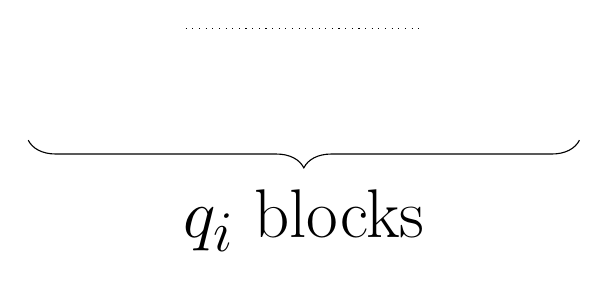
\begin{tikzpicture}
        \startb{0}{0}
        \middleb{3}{0}
        \draw[dotted] (5, 1) -- (8, 1);
        \middleb{8}{0}
        \startb{11}{0}
        \draw [decorate,decoration={brace,amplitude=10pt,mirror},xshift=0pt,yshift=-12pt]
        (3, 0) -- (10, 0) node [below,black,midway,yshift=-0.5cm]
        {\Huge $q_i$ blocks};
    \end{tikzpicture}
    }
    \caption{Transformation of \textit{Subset sum} element $q_i$}
    \label{fig:wells}
\end{figure}

When placing the first block it is evident that we have only two choices: place the $\mathbf{H}_H$ block column 2-3 of any well. This transform the chosen well from a closed to an open state. We then proceed to placing the middle $q_i$ blocks. When deciding the outcome of these placements the following lemmas are of use:\\

\begin{lem}
TODO: prove that the height doesn't change in the columns in phase 1. Important for second lemma.
\end{lem}

\bigbreak

\begin{lem}
\label{lem:permclose}
In phase 1, placing a $\mathbf{H}$ block in any other column than 4-5 in a well will make the same well permanently closed.
\end{lem}

\begin{proof}
In the first case, the well is closed. We can only place the $\mathbf{H}$ block in column 2-3. Since no cells are cleared as a result, column 1 to 4 are filled except for the top two rows. We therefore cannot place any block in these columns without a game over. Either the column right of column 5 is filled, or the gameboard has ended. Since column 4 is also filled, we cannot place any block in column 5. Thus the well is permanently closed.

In the second case, the well is open. Apart from column 4-5, the $\mathbf{H}$ block can only be placed in column 3-4. This does not clear any cells as a result. Thus with the same arguments as in the first case, the well is permanently closed.
\end{proof}

Since later in the proof it will become apparent that having a permanently closed well makes it impossible to construct a optimal trajectory sequence, lemma~\ref{lem:permclose} leaves us no choice but to place all $\mathbf{H}$ blocks in column 4-5 of the open well. Finally the last $\mathbf{H}_H$ block must be placed either in column 2-3 of a closed well, or column 3-4 of an open well, in order to not permanently close a well.

\begin{figure}[H]
    \centering
    \begin{subfigure}[b]{0.55\textwidth}
        \resizebox{\linewidth}{!}{
            \begin{tikzpicture}
                \welldefault{0}{0}
                \startb{1}{10}
                \welldefault{5}{0}
                \draw[dashed] (0, 0) -- (0, 12);
                \draw[dashed] (10, 0) -- (10, 12);
                \draw[dashed] (0, 0) -- (10, 0);
                \draw[->, line width=10pt] (11, 6) -- (14, 6);
                \wellopenwhole{15}{0}
                \welldefault{20}{0}
                \draw[dashed] (15, 0) -- (15, 12);
                \draw[dashed] (25, 0) -- (25, 12);
                \draw[dashed] (15, 0) -- (25, 0);
            \end{tikzpicture}
        }
        \caption{First block}
    \end{subfigure}

    \begin{subfigure}[b]{0.55\textwidth}
        \resizebox{\linewidth}{!}{
            \begin{tikzpicture}
                \wellopenwhole{0}{0}
                \middleb{3}{10}
                \welldefault{5}{0}
                \draw[dashed] (0, 0) -- (0, 12);
                \draw[dashed] (10, 0) -- (10, 12);
                \draw[dashed] (0, 0) -- (10, 0);
                \draw[->, line width=10pt] (11, 6) -- (14, 6);
                \wellopenwhole{15}{0}
                \cellw{18}{7}
                \cellw{18}{6}
                \welldefault{20}{0}
                \draw[dashed] (15, 0) -- (15, 12);
                \draw[dashed] (25, 0) -- (25, 12);
                \draw[dashed] (15, 0) -- (25, 0);
            \end{tikzpicture}
        }
        \caption{Middle blocks}
    \end{subfigure}

    \begin{subfigure}[b]{0.55\textwidth}
        \resizebox{\linewidth}{!}{
            \begin{tikzpicture}
                \wellopenwhole{0}{0}
                \cellw{3}{7}
                \cellw{3}{6}
                \startb{2}{10}
                \welldefault{5}{0}
                \draw[dashed] (0, 0) -- (0, 12);
                \draw[dashed] (10, 0) -- (10, 12);
                \draw[dashed] (0, 0) -- (10, 0);
                \node at (12.5, 6)
                {\Huge or};
                \wellopenwhole{15}{0}
                \cellw{18}{7}
                \cellw{18}{6}
                \welldefault{20}{0}
                \startb{21}{10}
                \draw[dashed] (15, 0) -- (15, 12);
                \draw[dashed] (25, 0) -- (25, 12);
                \draw[dashed] (15, 0) -- (25, 0);
            \end{tikzpicture}
        }
        \caption{Final block}
    \end{subfigure}

    \caption{Block placement in phase 1}
    \label{fig:placement}
\end{figure}

Assuming that no blocks has been place such that any well is permanently closed, the following invariants holds at the start of the sequence corresponding to $q_i$:

\begin{enumerate}
\item Either both of the wells are closed, or both of the wells are open.

\item Column 1, 3 and 5 in any well are unchanged from the initial gameboard. Column 2 is unchanged except from the top two rows (which may be black or empty).

\item Let $q_0 = 0$. This does not change the semantics of the givet \textit{Subset sum} instance. Then in total 
\begin{equation*}
    2 \left( i-1 \right) + \sum_{j=0}^{i-1} q_j
\end{equation*}
blocks have been placed.

\item Since each block placement clears exactly 4 cells
\begin{equation*}
    8 \left( i-1 \right) + 4 \sum_{j=0}^{i-1} q_j
\end{equation*}
cells have been cleared.

\item There exists: 
    \begin{equation*}
        M_1, M_2 \subseteq \{q_0, \ldots q_{i-1}\}, M_1 \cap M_2 = \varnothing, M_1 \cup M_2 = \{q_0, \ldots, q_{i-1}\}
    \end{equation*}
such that for any well $w \in \{1,2\}$ it holds that the rows in interval
    \begin{equation*}
        \left[ 2 \left( K-1 + \sum Q - \sum M_w \right) +1, 2 \left( K-1 + \sum Q \right) \right]
    \end{equation*}
consists of white cells in column 4, and the rows in interval
    \begin{equation*}
        \left[ 1, 2 \left( K-1 + \sum Q - \sum M_w \right) \right]
    \end{equation*}
consists of black cells in column 4.
\end{enumerate}

\begin{figure}[H]
    \centering
    \resizebox{!}{0.3\paperheight}{
    \begin{tikzpicture}
        \invariantchart{0}{0}
        \draw[dashed] (-1, 0) -- (6, 0);
        \draw[dashed] (-1, 6) -- (6, 6);
        \draw[dashed] (-1, 12) -- (6, 12);
        \draw[dashed] (-1, 20) -- (6, 20);
        \draw[dashed] (5, 0) -- (5, 22);
        \node at (0.5, -0.5) {\large 1};
        \node at (1.5, -0.5) {\large 2};
        \node at (2.5, -0.5) {\large 3};
        \node at (3.5, -0.5) {\large 4};
        \node at (4.5, -0.5) {\large 5};
        \draw [decorate,decoration={brace,amplitude=10pt},xshift=-12pt,yshift=0pt]
        (0, 0) -- (0, 6) node [left,align=right,black,midway,xshift=-1cm]
        {\huge $2 \left( K-1 \right)$ rows};
        \draw [decorate,decoration={brace,amplitude=10pt},xshift=-12pt,yshift=0pt]
        (0, 6) -- (0, 12) node [left,align=right,black,midway,xshift=-1cm]
        {\huge $2 \left( \sum Q - \sum M_w \right)$ rows};
        \draw [decorate,decoration={brace,amplitude=10pt},xshift=-12pt,yshift=0pt]
        (0, 12) -- (0, 20) node [left,align=right,black,midway,xshift=-1cm]
        {\huge $2 \sum M_w $ rows};
        \draw (3.5, 0.5) -- (7, 0.5) node [right, black, xshift=1cm] 
        {\huge row 1};
        \draw (3.5, 5.5) -- (7, 5.5) node [right, black, xshift=1cm, yshift=-0.5cm] 
        {\huge row $2 \left( K-1 \right)$};
        \draw (3.5, 6.5) -- (7, 6.5) node [right, black, xshift=1cm, yshift=0.5cm] 
        {\huge row $2 \left( K-1 \right) + 1$};
        \draw (3.5, 11.5) -- (7, 11.5) node [right, black, xshift=1cm, yshift=-0.5cm] 
        {\huge row $2 \left( K-1 + \sum Q - \sum M_w \right)$};
        \draw (3.5, 12.5) -- (7, 12.5) node [right, black, xshift=1cm, yshift=0.5cm] 
        {\huge row $2 \left( K-1 + \sum Q - \sum M_w \right) +1$};
        \draw (3.5, 19.5) -- (7, 19.5) node [right, black, xshift=1cm] 
        {\huge row $2 \left( \sum Q + K - 1 \right)$};
    \end{tikzpicture}
    }
    \caption{Depiction of invariants}
    \label{fig:invariant}
\end{figure}

When every block sequence corresponding to the elements of $Q$ has been placed, $a$ elements has been transformed. For all purposes of this proof this is equivalent to being at the start of the sequence corresponding to $q_{a+1}$, even though strictly speaking no such element is given. Thus $i = a+1$ and from the invariants we obtain:

\begin{enumerate}
\item Still holds.
\item Still holds.
\item In total
\begin{equation*}
    2a + \sum Q
\end{equation*}
blocks have been placed.

\item In total
\begin{equation*}
    8a + 4 \sum Q
\end{equation*}
cells have been cleared.

\item There exists:
\begin{equation*}
    M_1, M_2 \subseteq Q, M_1 \cap M_2 = \varnothing, M_1 \cup M_2 = Q
\end{equation*}
such that for any well $w \in \{1,2\}$ it holds that the rows in interval
\begin{equation*}
        \left[ 2 \left( K-1 + \sum Q - \sum M_w \right) +1, 2 \left( K-1 + \sum Q \right) \right]
    \end{equation*}
consists of white cells in column 4, and the rows in interval
    \begin{equation*}
        \left[ 1, 2 \left( K-1 + \sum Q - \sum M_w \right) \right]
    \end{equation*}
consists of black cells in column 4.
\end{enumerate}


\subsubsection{Phase 2}
\label{subsub:phasetwo}
In this phase a single $\mathbf{X}_H$ block is generated. From the invariants presented in~\ref{subsub:phaseone} we know that the top of the two wells must be in one of the two states presented in~\autoref{fig:openclosed}. Thus the only non-losing option is to place the $\mathbf{X}_H$ block in such a way that it closes one of the wells permanently. Note that if any well was permanently closed before this phase, this placement renders both of the wells permanently closed, making it impossible to clear any more cells during the game.

\begin{figure}[H]
    \centering
    \begin{subfigure}[b]{0.35\textwidth}
        \resizebox{\linewidth}{!}{
            \begin{tikzpicture}
            \ptwoclosed{0}{0}
            \stopb{1}{8}
            \draw[dashed] (0, 0) -- (0, 10);
            \draw[dashed] (5, 0) -- (5, 10);
            \draw[->, line width=5pt] (6, 5) -- (9, 5);
            \ptwoclosed{10}{0}
            \draw[dashed] (10, 0) -- (10, 10);
            \draw[dashed] (15, 0) -- (15, 10);
            \stopb{11}{6}
            \end{tikzpicture}
        }
        \caption{}
    \end{subfigure}
    \hspace{0.05\textwidth}
    \begin{subfigure}[b]{0.35\textwidth}
        \resizebox{\linewidth}{!}{
            \begin{tikzpicture}
            \ptwoopen{0}{0}
            \stopb{2}{8}
            \draw[dashed] (0, 0) -- (0, 10);
            \draw[dashed] (5, 0) -- (5, 10);
            \draw[->, line width=5pt] (6, 5) -- (9, 5);
            \ptwoopen{10}{0}
            \stopb{12}{6}
            \draw[dashed] (10, 0) -- (10, 10);
            \draw[dashed] (15, 0) -- (15, 10);
            \end{tikzpicture}
        }
        \caption{}
    \end{subfigure}

    \begin{subfigure}[b]{0.35\textwidth}
        \resizebox{\linewidth}{!}{
            \begin{tikzpicture}
            \ptwoopen{0}{0}
            \stopb{3}{8}
            \draw[dashed] (0, 0) -- (0, 10);
            \draw[dashed] (5, 0) -- (5, 10);
            \draw[->, line width=5pt] (6, 5) -- (9, 5);
            \ptwoopen{10}{0}
            \cellw{13}{6}
            \cellb{13}{7}
            \draw[dashed] (10, 0) -- (10, 10);
            \draw[dashed] (15, 0) -- (15, 10);
            \end{tikzpicture}
        }
        \caption{}
    \end{subfigure}

    \caption{Possible cases in phase 2}
    \label{fig:placement}
\end{figure}


\subsection{Conclusion}

Corollary~\ref{cor:np} and theorem~\ref{thm:nphard} directly yields the following corollary: \\

\begin{cor}
The (offline, no-rotation, acyclic) k-cleared-cells problem is NP-complete.
\end{cor}


\section{Discussion}
\label{discussion}

\subsection{Rotations}

The two main ways the player can control the blocks in the original Lumines video game is to rotate and move the them left and right. The simplified mode presented in thisis does not consider rotation of the blocks, meaning an important aspect of the game is not considered. It was the original goal of the report to formulate and research a model which included rotations, but time constraints did not permit this. Intuitively rotation should have some impact on the hardness of the game. The authors found it harder to find a reduction from subset sum to a Lumines model where rotations were considered. This suggests the possibility of the model including rotations to be easier than NP-hard. However this does not have to be the case. Rotations may be harder if it could be proven that an algorithm would have to consider all possible ways to build terrain in this model. It is imporant to emphasize that nothing has been found that proofs the impact of rotations on the computational complexity of the model. Therefore this should be examined in future work to get a better understanding of the video game's complexity.

\subsection{Sweep-line}

In Lumines the sweep-line moves in constant speed from left to right. The marked squares are then cleared as the sweep-line scans the cells in their respective marked squares. The simplified Lumines model that is presented in this paper uses an instant sweep-line, in which the cells are marked and cleared simultaneously when a square is formed. This is similar to how rows are cleared in Tetris, but not the most accurate representation of how the sweep-line works in Lumines. There is probably room for improvement in making a more accurate model of the sweep-line game mechanic. For example, every $n\text{th}$ block that is fixed could trigger the clearing of marked cells. The less accurate model in this report was chosen since it was more suitable to work with given the time limit of the project. It is however important to note that the amount of cells that can be cleared in a given sequence can vary dramatically between different models of the sweep-line (see \textbf{todo figure showing this}). Therefore, in future work, inquires into the impact of the chosen sweep-line model on the computational complexity would be a promising area of research.

\subsection{Online Lumines}

In this report the offline version of Lumines has been considered. This is similar to previous studies on Match-three games and Tetris, where offline versions of the respective games have been considered. In these reports the authors argue that if the computational complexity of a property can be shown in the offline version of the games, intuitively it corresponding computational complexity in the online version should be as hard or harder. According to Demaine, Hoffman and Holzer, ``...it is only easier to play Tetris with complete knowledge of the future, so the difficulty of playing the offline version suggests the difficulty of playing the online version'' \cite[p. 2]{tetris}. If this statement is true it is probable that this is also the case for Lumines. However none of the examined papers present any proof that this is the case, either in the general case or specifically to their respective considered games. Therefore the online version of Lumines should be examined in the future to research if such a proof can be conducted.

\subsection{Subset sum}

None of the reductions encountered in examined material utilized the subset sum problem. The most commonly found problem to reduce from was the 3-SAT problem. It is the author's beliefs that this is the first paper concerning video game complexity using the subset sum problem. Although the nature of NP-completeness permits all NP-complete problem to be equally valid for use in reductions, some problems are inherently easier to reduce from than others depending on the problem to reduce to. The results from this report shows promising signs that subset sum is suitable problem to reduce from when examining other 2D stacking puzzle games. 

\printbibliography
\newpage
\begin{appendices}
\section{Special case of the reduction}
\label{specialcasereduction}

In \ref{phase3} we mention a special case of the reduction where the player has chosen to put all $\mathbf{H}$ blocks from phase 1 in the same well and then closed this well during phase 2. The following will show that if this case is reached it is not possible to create an optimal clearing of cells in the given game.

\subsection*{Phase 3}
Being in the state explained above gives the player the option to clear the black cells in column 3-4 with a $\mathbf{MB}$ block, clearing 6 cells in total. When the player places the $\mathbf{MW}$ block, she can choose either to place it in column 2-3 or in column 3-4. However this is irrelevant to the question of whether it is possible to clear an optimal amount of cells, since the two options clear the same amount of cells and result in the same gameboard.

Because two extra cells are cleared in this phase, the total amount of cells cleared after phase 3 is at most $8a + \sum Q + 12$ cells in this special case.

\subsection*{Phase 4 and 5}

Phase 4 and 5 can be seen as the same phase in this special case. During this 4-5 phase the player places $\sum Q - 1$ $\mathbf{LB}$ blocks on the gameboard. To maximize the amount of cleared cells she is required to place the blocks in column 4-5. In column 4 there are $2 \sum \left( Q + K - 1 \right) - 1$ cells, which means the maximum amount of cleared cells during this phase is $ 4 \left( \sum Q - 1 \right)$. This leaves $2K-1$ black cells in column 4.

\subsection*{Summing of the phases}

Given the information in previous sections, the maximum amount of cleared cells in this special case is

\begin{align*}
  & 8a + \sum Q + 12 + 4 \left( \sum Q - 1 \right) \\
= \; & 8a + 5 \sum Q + 8
\end{align*}

Compared to the general case given for $K > 1$, given in \ref{sub:nphard}, this case yields fewer possible cleared cells.

\begin{equation*}
8a + 5 \sum Q + 8 < 8a + 5 \sum Q + 4 + 4K
\end{equation*}

Therefore, the special case can never result in an optimal amount of cleared cells.

\end{appendices}

\end{document}
